\chapter{Leader Election Algorithm}

\section{System Model}
In this section, we explain the local variables used in our leader election algorithm. The pseudocode for the algorithm is presented in Figures 3.1, 3.2 and 3.3. An overview and sample execution is given in Section 3.1. In the analysis, variable v of node i will be indicated as v i.

Each node i keeps an array of heights, height i , with an entry for itself and for each of its neighbors, in which it stores the most recent height information that it has received for those nodes.

Each height is a 7-tuple, with the following components:
\begin{enumerate}
\item $\tau$ , a nonnegative timestamp that is either 0 or the time when the current search for an alternate path to the leader was initiated
\item oid, a nonnegative value that is either 0 or the id of the node that started the current search
\item r, a bit that is set to 0 when the current search is initiated and set to 1 when the current search hits a deadend
\item δ , an integer that is set to ensure that links are directed appropriately to neighbors with the same first three components
\item nlts, a nonpositive timestamp whose absolute value is the time when the current leader was elected
\item lid, the id of the current leader
\item id, the id of the node
\end{enumerate}
Components ( τ , oid, r) are referred to as the reference
level, or RL; ( τ , oid) alone are referred to as the reference
level prefix; and (nlts, lid) is referred to as the leader pair
or LP. The components of entry k in height i are referred to
as ( τ k , oid k , r k , δ k , nlts k , lid k , k) in the pseudocode.

Nodes communicate over links during the algorithm ex-
ecution by sending Update messages. Each message con-
tains the height tuple and the logical clock timestamp of the
sending node. The link between node i and one of its neigh-
boring nodes j is considered by i to be outgoing (directed
from i to j) if and only if height i [i] > height i [ j]. That is,
node i uses the information in its local state concerning it-
self and node j to determine (its view of) the direction of the
link to j. Because of message delays, it is not necessarily
the case that i and j have consistent views of the direction
of the link between them.

Other events that occur at a node are formations
(LinkUps) and failures (LinkDowns) of links. Suppose the
most recent indication that node i has received concerning
the link between itself and node j is a LinkUp. If i has re-
ceived a message from j since that LinkUp, then i considers
j as one of its neighbors, and stores the id of j in its local
variable N i . If i has not yet received a message from j, then
the link is considered as still forming, and i stores the id of j
in its local variable forming i ; j is not considered a neighbor
of i (yet).

Nodes have no access to global time, but, instead, each
of them has a local logical clock [11]. A logical clock is
a non-negative integer, initially 0. Logical clocks can be
updated in two possible ways, depending on the type of the
event occurring at a node. If a LinkUp or a LinkDown event
occurs at a node, its logical clock is incremented by 1. Oth-
erwise, if a node receives an Update message, the logical
clock is set to one more than the maximum of the node’s
current logical clock value and the timestamp included in
the message. This way, we ensure that for each node, the
value of its logical clock is non-decreasing for each subse-
quent event. The logical clock of a node is referred to as LC
in the pseudocode.

Given an initial connected communication graph G =
(V, E), with V corresponding to the set of nodes and E to
the set of communication links that are up, the initial state
of each node i is defined as follows 1 .
\begin{enumerate}
\item forming i is empty
\item N i contains the id of every node j such that the vertices
in V corresponding to i and j are neighbors in G
\item height i [i] = (0, 0, 0, δ i , 0, l, i), where l is the id of a
fixed node in i’s connected component, the current
leader
\item for each neighbor j of i, height i [ j] = height j [ j] (i.e., i
has accurate information about j’s height)
\item LC i = 0 (i.e. the logical clocks of all nodes are initially
set to 0).
\end{enumerate}
Furthermore, for each node i, δ i equals the distance from i
to l; this condition ensures that every node has a directed
path to l.
Next we define the conditions under which a node con-
siders itself to be a sink.
\begin{itemize}
\item SINK = ((LP i j = LP ii ∀ j ∈ N i ) and (height i [i] <
min{height i [ j] ∀ j ∈ N i }) and (lid ii , i)). This pred-
icate is true when, according to i’s local state, i is not
a leader, has all neighbors with the same LP, and has
no outgoing links. If node i has links to any neighbors
with different LPs, i is not considered a sink, regard-
less of the directions of those links.
\end{itemize}
\section{Overview of Algorithm}
We depict the network as a DAG in which each bidirec-
tional communication link points from a node with lexico-
graphically higher height to another node with lexicograph-
ically lower height. Nodes send algorithm messages only
when they change the contents of their height tuple. The
contents of the height tuple at a particular node are changed
only when the node elects itself a leader, when it changes its
current leader, or when it loses its last outgoing link to its
current leader. The network is quiescent when there is no
message in transit on any link. Messages that do not cause
a node to lose its last outgoing link to its current leader or
to change its current leader result only in a change to the
internal data that node keeps about its neighbors’ heights.
Figure 3.4 shows a sample execution of the algorithm.
Each part (a)–(h) is discussed below.
\begin{enumerate}[label=\alph *)]
\item A quiescent network is a leader-oriented DAG in
which node H is the current leader. The height of each
node is displayed in parenthesis. Link direction in this
figure is shown using solid-headed arrows and mes-
sages in transit are arrows with outlined heads super-
imposed on the links that point from message sender
to receiver.
\item When non-leader node G loses its last outgoing link
due to the loss of the link to node H, G increments
its logical clock by 1, executes subroutine START -
N EW R EF L EVEL and takes on RL (1,G,0) and δ = 0.
Then node G sends messages with its new height to all
its neighbors. By raising its height in this way, G has
started a search for leader H.
\item Nodes D, E, and F receive the messages sent from node
G, messages that cause each of these nodes to take on
RL (1,G,0), set its δ to −1, ensuring that its height is
lower than G’s but higher than the other neighbors’.
Moreover, each of these nodes also updates its logical
clock to 2. Then D, E and F send messages to their
neighbors.
\item Node B has received messages from both E and D with
the new RL (1,G,0), and C has received a message
from F with RL (1,G,0); as a result, B and C take on
RL (1,G,0) with δ set to −2, update their logical clocks
to 3 and send messages. Additionally, as a result of the
messages sent by D, E, and F, node G updates its logi-
cal clock to 3.
\item Node A has received message from both nodes B and
C. In this situation, node A is connected only to nodes
that are participating in the search started by node G
for leader H. In this case, node A “reflects” the search
by setting the reflection bit in the (1,G,*) reference
level to 1, resetting its δ to 0, and sending its new
height to its neighbors. Moreover, nodes A, D, E, and
F update their clocks to 4.
\item Nodes B and C take on the reflected reference level
(1,G,1) and set their δ to −1, causing their heights to
be lower than A’s and higher than their other neigh-
bors’. They also update their logical clocks to 5 and
send their new heights to their neighbors.
\item Nodes D, E, and F act similarly as B and C did in part
(f), but set their δ variables to −2. As a result from
the messages sent by B and C, nodes A, D, E, and F
update their logical clocks to 6.
\item When node G receives the reflected reference level
from all its neighbors, it knows that its search for H is
in vain. G updates its logical clock to 7 and then elects
itself. The new LP (-7,G) then propagates through the
component, updating nodes’ logical clocks along the
way, assuming no further link changes occur; eventu-
ally each node has RL (0,0,0) and LP (-7,G), with D,
E and F having δ = 1, B and C having δ = 2, and A
having δ = 3.
\end{enumerate}

%\newpage
\begin{figure}[hbtp]
\textbf{When $ChannelDown_uv$ event occurs}

\begin{enumerate}
\item \quad $ N := N\backslash \left\lbrace v\right\rbrace $
\item \quad $ forming := forming \backslash \left\lbrace v\right\rbrace $
\item \quad \textbf{if} $ (N = \emptyset )$
\item \quad \quad $ELECTSELF$
\item \quad \quad send Update(heigth[u]) to all $ w\in forming$
\item \quad \textbf{else if}(SINK)
\item \quad \quad $STARTNEWREFLEVEL$
\item \quad \quad send Update(heigth[u]) to all $w\in (N \cup forming)$
\item \quad \textbf{else if} $(j=pred_i)$
\item \quad \quad $pred_i=min \left\lbrace k \quad \vert \quad k\in N_i \quad and \quad \delta_k = \delta_j \right\rbrace$
\item \quad \textbf{end if}

\end{enumerate}
\end{figure}

\begin{figure}[hbtp]
\centering
\includegraphics[scale=.75]{../../Pictures/algorithm_2.png}
\caption{Code triggered by link changes.}
\end{figure}
\begin{figure}[hbtp]
\centering
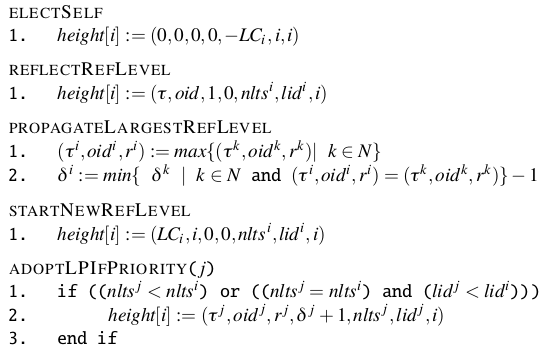
\includegraphics[scale=.75]{screenshot_3.png}
\caption{Subroutines}
\end{figure}

\begin{figure}[hbtp]
\centering
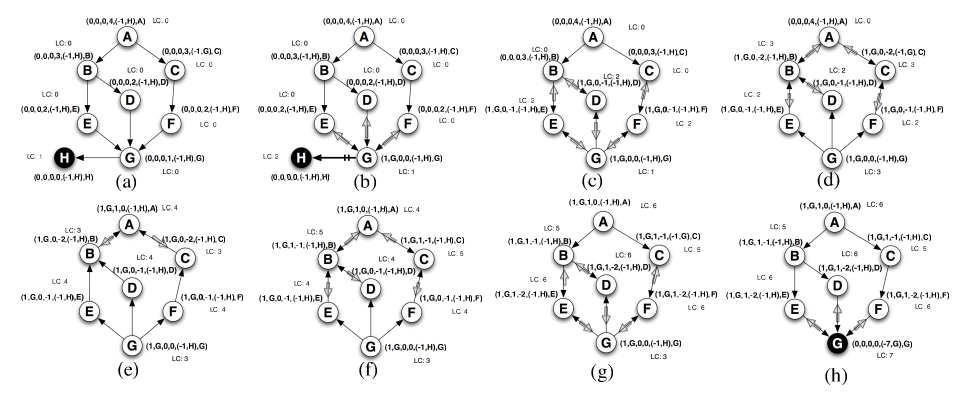
\includegraphics[scale=.5]{screenshot_1.png}
\caption{Simple execution when leader H becomes disconnected (a), with time increasing from (a)–
(h). With no other link changes, every node in the connected component will eventually adopt G as
its leader.}
\end{figure}




